\documentclass[acmtog]{techreportacmart}

\usepackage{booktabs} % For formal tables


\usepackage[ruled]{algorithm2e} % For algorithms
\renewcommand{\algorithmcfname}{ALGORITHM}
\SetAlFnt{\small}
\SetAlCapFnt{\small}
\SetAlCapNameFnt{\small}
\SetAlCapHSkip{0pt}
\IncMargin{-\parindent}

% Copyright
\setcopyright{none}

\settopmatter{printacmref=false, printccs=false, printfolios=true}
\citestyle{acmauthoryear}
\setcitestyle{square}

% Document starts
\begin{document}
% Title portion
\title{Report: Deep Learning Methods for Reynolds-Averaged Navier-Stokes Simulations of
Airfoil Flows \\ Master-Seminar - Deep Learning in Physics} 
\author{Julian Hohenadel}
\affiliation{%
  \institution{Technical University of Munich}
}

\renewcommand\shortauthors{Hohenadel}

\begin{abstract}
This report aims to critically assess a deep learning approach to infer Reynolds-Averaged Navier-Stokes solutions. Following the thoughts of \cite{Thuerey20} a fully convolutional U-Net architecture is used to classify the performance on deriving pressure and velocity fields and their distributions. With an evaluation of different hyperparameter regarding network and training data size, the best models yield a mean error relative to pressure and velocity channels of less than 3\% on a test set containing 90 unseen airfoil shapes. \cite{Thuerey20} states that due to this generic approach other PDE boundary value problems on Cartesian grids can also be tackled with this setup. In this report different adaptations of the network architecture are compared to each other with different data normalization in form of vector norms. Lastly the architecture is used to predict wave propagation on shallow water governed by the Saint-Venant equations.
\end{abstract}

%
% End generated code
%

\keywords{RANS, Reynolds-Averaged Navier-Stokes, CNN, U-Net, FCNN, PDE, CFD, Cartesian grid, pressure, velocity, airfoil, flow prediction, Eulerian field functions}


\thanks{This report is a part of the lecture, Master-Seminar - Deep Learning in
  Computer Graphics, Informatics 15, Technical University of Munich.}


\maketitle

\section{Introduction}
Since the last few years machine learning as well as deep learning in the form 
of neural networks enjoy great popularity. Their broad spectrum of application 
fields paired with the competitiveness of the researchers and fast available hardware (GPUs) 
allow the scientific community to squeeze out every bit of performance of their 
neural networks. \\
This hype also affects the computational fluid dynamics (CFD) field as \cite{viquerat2019}
shows with an exponential growth in published papers over the last 20 years.
Solving flow prediction problems traditionally is coupled with a deep understanding 
of physics and modeling these complex physical constrains. A neural network with a 
high enough capacity is capable to capture these high-dimensional, nonlinear constrains.
Neural networks are universal approximators \cite{Approximation} i.e. there is always a
trade-off regarding accuracy to the ground truth function (actual dynamics) and the 
number of parameter in the network. \\
\cite{Thuerey20} explains the first goal is to alleviate concerns regarding achievable accuracy
and analyzability of deep learning approaches by showing a relation between accuracy and
changes in the  hyper-parameter of a network.
As the second goal the paper provides a testing environment hosted on Github. 
The code is clean and easy to read. Training data is also available which is 
a jump start for own experiments with computational fluid dynamics. Different training
dataset sizes and a flexible network capacity prevents long training time which can arise
from a potential hardware bottleneck. Using Google Colab different kinds of ReLu activation functions and their impact on the networks accuracy are compared based on their mean errors regarding pressure, velocity and combined. Data preprocessing is one of the most important aspects to make the training fast and converge to good minima. For that reason different vector and pseudo norms are used to profit from dimensionless training data with different scalings. To prove that this generic setup as \cite{Thuerey20} claims is applicable to other partial differential equations (PDE) boundary value problems the network architecture is used to train on infering the Saint-Venant equations, which \cite{Fotiadis2020} uses for the modeling of surface wave propagation.

\section{Background}
Reynolds-averaged Navier-Stokes (RANS) equations are used for the modeling of turbulent incompressible flows \cite{Alfonsi}. \\
The Navier-Stokes equation is a nonlinear partial differential equation which can be seen as Newtons's 2nd law of motion \cite{BISTAFA2018}:
% Numbered Equation
\begin{equation}
\label{eqn:01}
\frac{\partial{u}}{\partial{t}} + u \cdot \nabla u = g - \frac{1}{\rho} \nabla p + \nu \nabla^{2}u
\end{equation}
where $u$ is the velocity vector, $g$ is the acceleration vector due to a body force, $p$ is pressure, 
$\nu$ is the kinematic viscosity and $\rho$ is the density. \cite{BISTAFA2018} rewrites the left side of the equation as the particles acceleration and the right side as the external forces that affect the particle per unit of mass which yields Newtons's 2nd law of motion. The idea behind RANS is Reynolds decomposition which splits dependent model variables into a mean and fluctuating part \cite{Alfonsi}. The Reynolds number $Re$ is a dimensionless constant which is needed for the calculation of turbulence models. Depending on the magnitude of the Reynolds number the flow ranges from laminar to turbulent \cite{lissaman1983}. The angle of attack on an airfoil as well as the Reynolds number are important parameter for the creation of the physical model because they affect lift and drag coefficients \cite{lissaman1983}. 

\section{Method}
In the following the methodology used by \cite{Thuerey20} to infer the RANS solutions is summarized and extended by experiments evaluated for this report. For consistency reasons the structure is kept equal to the original paper.

\subsection{Data Generation}
The UIUC database \cite{airfoil} holds a variety of airfoil shapes, shown in Figure~\ref{fig:one}, which are used to generate training data. The provided data is only a 2D coordiante representation of the airfoil shape. To aquire the ground truth velocity and pressure maps the open source package OpenFOAM is used which contains solvers for CFD problems. The range of Reynolds numbers $[0.5, 5] \cdot 10^{6}$ used for generating the ground truth indicates turbulent airflow. Also an angle of attack of $\pm 22.5$ degrees is used. RANS turbulence models distinguish between different classes \cite{Alfonsi}. In this case the one-equation model is used. The solutions are cropped to a resolution of $128x128$ pixels arround the airfoil to speed up training while keeping the most relevant information. A test set is generated seperately with unseen airfoil shapes.

% Figure
\begin{figure}[H]
  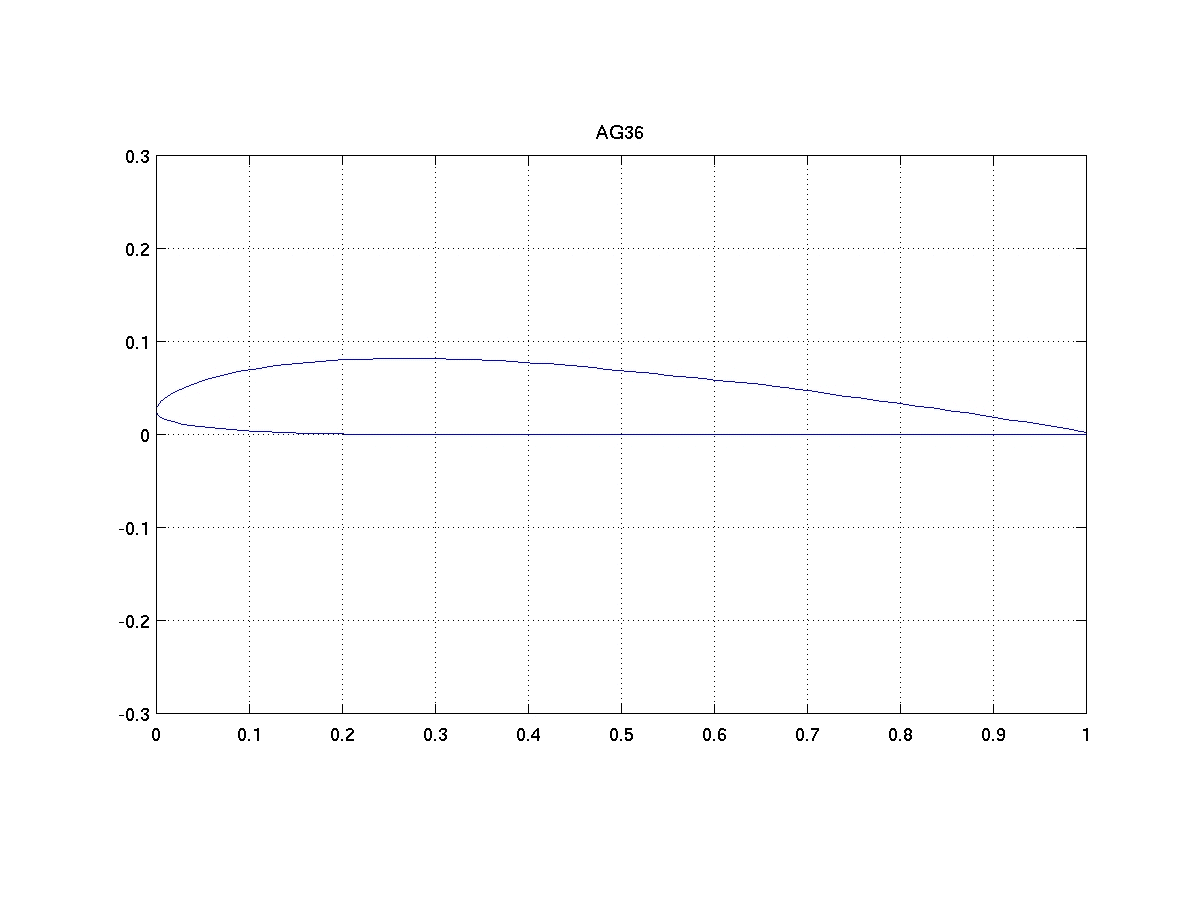
\includegraphics[width=.4\textwidth]{figures/uiuc_sample}
  \vspace*{-10mm}
  \caption{A sample airfoil shape in 2D.}
  \label{fig:one}
\end{figure}

\subsection{Pre-processing}
One training data sample consists of $3$ $128x128$ grids wrapped into a tensor. The channels are a bit mask representing the position and shape of the airfoil, $x$ and $y$ velocity. Inside the airfoil shape all elements contain $0$ in the velocity fields. The velocity maps are initialized with differently scaled freestream velocity vectors which have the corresponting Reynolds number for the sample encoded in them with respect to the magnitude of the elements. For the infered solution of the neural network the shape stays the same as the input. \cite{Thuerey20} use the solution obtained from OpenFOAM as ground truth with channels split into pressure, $x$ and $y$ velocity. The first normalization step is to divide the  ground truth data with the magnitude of the freestream velocity (default: L2 vector norm). The pressure channel is divided with the vector norm squared to make the data dimensionless. This originates in the physical unit of pressure: In an incompressible model the density is constant so to make the pressure dimensionsless it needs to be divided with the squared velocity. \\

% Table
\begin{table}[h]
\caption{Norm comparision wrt. error, L2 default (in \%).}
\label{tab:one}
\begin{center}
\begin{tabular}{l|l|l|l|l}
  \toprule
  Norm   & pressure   &	velocity    & combined \\
  \bf L1	 & \bf 14.19	  & \bf 2.251		& \bf 2.646    \\
  L2	 & 14.76	  & 2.291		& 2.780	   \\
  L inf	 & 15.09	  & 2.348		& 2.865	   \\
  L 0.25 & 31.03	  & 3.106		& 3.272	   \\
  L 0.5  & 15.64	  & 2.448		& 2.705	   \\
  L 0.75 & 31.03	  & 3.106		& 3.272	   \\	
  \bottomrule
\end{tabular}
\end{center}
\bigskip\centering
\footnotesize L1 normalization achieves the best error rates (lower is better). \\
Trained on \cite{Thuerey20} U-net implementation with $1.9 \cdot 10^{6}$ weights. \\
Used seeds for training: $0$, $2^{10}$, $2^{20}$, $2^{30}$
\end{table}%

Table~\ref{tab:one} shows how different vector norms which are only used for normalization of the target data in the pre-processing step change the averaged error of neural networks which are all trained under the same conditions and capacity. Figure~\ref{fig:three} visualizes the relations of the p-norms on the unit circle: $L1 \geq L2 \geq L_{inf}$\\
Interestingly the same inequality relation holds for every error channel shown in Table~\ref{tab:one} as well. The other norms are quasi norms because they violate the required convexity but follow the same definition for a vector $x$: 

% Numbered Equation
\begin{equation}
\label{eqn:01}
||x||_p := {\left( \sum_{i=0}^{n} |x_i|^p \right)}^{\frac{1}{p}}
\end{equation}

Surprisingly L$0.25$ and L$0.75$ normalization hold exactly the same results, although the absolute norm values on the same sample differ vastly. They also fail to infer target pressure values by arround $2x$ when compared with the other norms. \\

% diff_layer_0_bn_weight
\begin{figure}[H]
  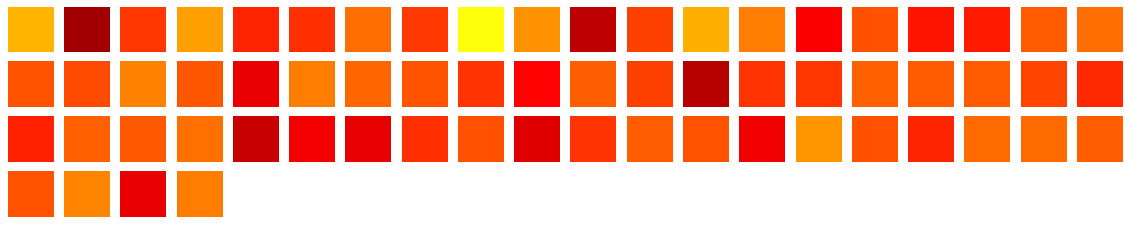
\includegraphics[width=.3\textwidth]{figures/weights_visualized/diff_layer_0_bn_weight.png}
  \caption{Batchnorm weight difference between L1 and L2 normalization.}
  \label{fig:five}
\end{figure}

% diff_layer_0_bn_bias
\begin{figure}[H]
  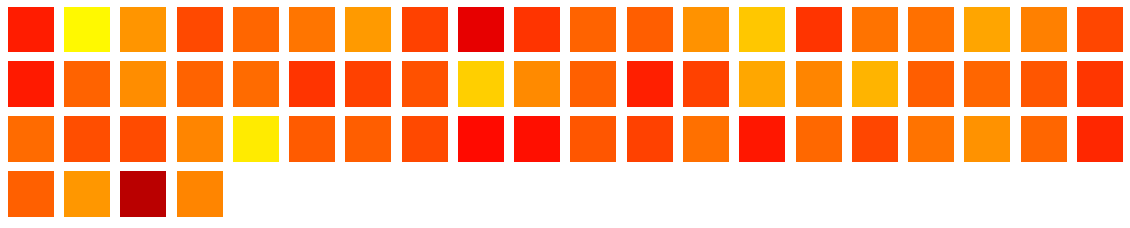
\includegraphics[width=.3\textwidth]{figures/weights_visualized/diff_layer_0_bn_bias.png}
  \caption{Batchnorm bias difference between L1 and L2 normalization.}
  \label{fig:six}
\end{figure}

% diff_layer_1_conv
\begin{figure}[H]
  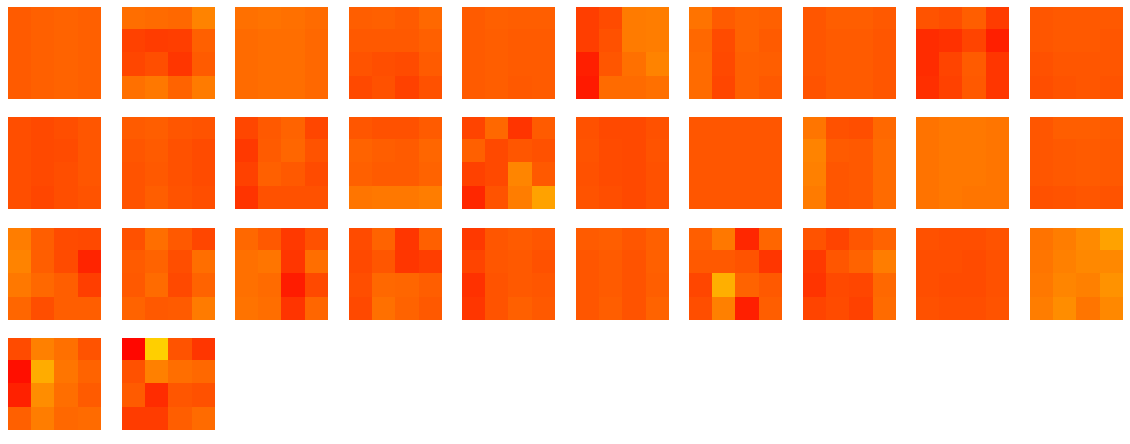
\includegraphics[width=.3\textwidth]{figures/weights_visualized/diff_layer_1_conv.png}
  \caption{Convolution weight (1. layer) difference between L1 and L2 normalization}
  \label{fig:seven}
\end{figure}

Additionally to norm based normalization the pressure channel is shifted into the origin by subtraction the pressure mean for each sample respectively. By doing this the network does not have to waste ressources on compensating for an off centered pressure map. Lastly \cite{Thuerey20} clamps each channel into an $[-1, 1]$ interval to ensure a maximum of numerical precision.

\subsection{Neural Network Architecture}
\cite{Thuerey20} use a modified version of the U-Net architecture proposed by \cite{ronneberger2015} (Figure~\ref{fig:two}) which was first successfully used for biomedical image segmentation.
The U-Net architecure consists of two parts. The left side of the "U" functions as an encoder. It captures the context of the image. While width and height of the image get smaller the depth of the channels increases. The right side acts as a decoder. It upsamples the feature maps to recover spatial locations. The behavior of the image size and depth is contrary to the encoder part. Every block is implemented similary: activation function (leaky ReLu in encoder, ReLu in decoder), convolution layer, batch normalization and finally dropout for regularization \cite{Thuerey20}. Without the help of skip connections information captured in the initial layers of the U-Net which is needed for reconstruction in the decoding part may get lost. This can be avoided by concatenating horizontal aligned blocks.


Only created not in use
\begin{table}[h]
\caption{Activation function comparision wrt. error (in \%).}
\label{tab:two}
\begin{center}
\begin{tabular}{l|l|l|l|l}
  \toprule
  Norm   & pressure   &	velocity    & combined \\
  \bf Std	 & \bf 14.76	  & \bf 2.291		& \bf 2.780	   \\
  PReLu	 & 18.17	  & 2.453		& 2.871	   \\
  ReLu	 & 34.13	  & 3.369		& 3.547	   \\
  \bottomrule
\end{tabular}
\end{center}
\bigskip\centering
\footnotesize The activation functions proposed by \cite{Thuerey20} achieve \\ the best error rates (lower is better).
\end{table}%

\subsection{Supervised Training}

\begin{comment}

\subsection{Data preparation (Normalization)}
\subsection{U-Net Architecture}
\subsection{Training}
\subsection{Accuracy}
\subsection{Performance}

\section{Prelu, performance, weight visual, test with mean in leaky}
\section{Normalization Norms}
\section{Conv Filter - Gap between Params in NN}
\section{Transfer to wave propagation}

\section{Discussion}

\section{Conclusion}
\end{comment}

Lorem ipsum dolor sit amet, consetetur sadipscing elitr, sed diam nonumy eirmod tempor invidunt ut labore et dolore magna aliquyam erat, sed diam voluptua. At vero eos et accusam et justo duo dolores et ea rebum. Stet clita kasd gubergren, no sea takimata sanctus est Lorem ipsum dolor sit amet. Lorem ipsum dolor sit amet, consetetur sadipscing elitr, sed diam nonumy eirmod tempor invidunt ut labore et dolore magna aliquyam erat, sed diam voluptua. At vero eos et accusam et justo duo dolores et ea rebum. Stet clita kasd gubergren, no sea takimata sanctus est Lorem ipsum dolor sit amet. Lorem ipsum dolor sit amet, consetetur sadipscing elitr, sed diam nonumy eirmod tempor invidunt ut labore et dolore magna aliquyam erat, sed diam voluptua. At vero eos et accusam et justo duo dolores et ea rebum. Stet clita kasd gubergren, no sea takimata sanctus est Lorem ipsum dolor sit amet.   

Duis autem vel eum iriure dolor in hendrerit in vulputate velit esse molestie consequat, vel illum dolore eu feugiat nulla facilisis at vero eros et accumsan et iusto odio dignissim qui blandit praesent luptatum zzril delenit augue duis dolore te feugait nulla facilisi. Lorem ipsum dolor sit amet, consectetuer adipiscing elit, sed diam nonummy nibh euismod tincidunt ut laoreet dolore magna aliquam erat volutpat.   

Ut wisi enim ad minim veniam, quis nostrud exerci tation ullamcorper suscipit lobortis nisl ut aliquip ex ea commodo consequat. Duis autem vel eum iriure dolor in hendrerit in vulputate velit esse molestie consequat, vel illum dolore eu feugiat nulla facilisis at vero eros et accumsan et iusto odio dignissim qui blandit praesent luptatum zzril delenit augue duis dolore te feugait nulla facilisi.   

Nam liber tempor cum soluta nobis eleifend option congue nihil imperdiet doming id quod mazim placerat facer possim assum. Lorem ipsum dolor sit amet, consectetuer adipiscing elit, sed diam nonummy nibh euismod tincidunt ut laoreet dolore magna aliquam erat volutpat. Ut wisi enim ad minim veniam, quis nostrud exerci tation ullamcorper suscipit lobortis nisl ut aliquip ex ea commodo consequat.   

Duis autem vel eum iriure dolor in hendrerit in vulputate velit esse molestie consequat, vel illum dolore eu feugiat nulla facilisis.   

At vero eos et accusam et justo duo dolores et ea rebum. Stet clita kasd gubergren, no sea takimata sanctus est Lorem ipsum dolor sit amet. Lorem ipsum dolor sit amet, consetetur sadipscing elitr, sed diam nonumy eirmod tempor invidunt ut labore et dolore magna aliquyam erat, sed diam voluptua. At vero eos et accusam et justo duo dolores et ea rebum. Stet clita kasd gubergren, no sea takimata sanctus est Lorem ipsum dolor sit amet. Lorem ipsum dolor sit amet, consetetur sadipscing elitr, At accusam aliquyam diam diam dolore dolores duo eirmod eos erat, et nonumy sed tempor et et invidunt justo labore Stet clita ea et gubergren, kasd magna no rebum. sanctus sea sed takimata ut vero voluptua. est Lorem ipsum dolor sit amet. Lorem ipsum dolor sit amet, consetetur sadipscing elitr, sed diam nonumy eirmod tempor invidunt ut labore et dolore magna aliquyam erat.   

Consetetur sadipscing elitr, sed diam nonumy eirmod tempor invidunt ut labore et dolore magna aliquyam erat, sed diam voluptua. At vero eos et accusam et justo duo dolores et ea rebum. Stet clita kasd gubergren, no sea takimata sanctus est Lorem ipsum dolor sit amet. Lorem ipsum dolor sit amet, consetetur sadipscing elitr, sed diam nonumy eirmod tempor invidunt ut labore et dolore magna aliquyam erat, sed diam voluptua. At vero eos et accusam et justo duo dolores et ea rebum. Stet clita kasd gubergren, no sea takimata sanctus est Lorem ipsum dolor sit amet. Lorem ipsum dolor sit amet, consetetur sadipscing elitr, sed diam nonumy eirmod tempor invidunt ut labore et dolore magna aliquyam erat, sed diam voluptua. At vero eos et accusam et justo duo dolores et ea rebum. Stet clita kasd gubergren, no sea takimata sanctus.   

Lorem ipsum dolor sit amet, consetetur sadipscing elitr, sed diam nonumy eirmod tempor invidunt ut labore et dolore magna aliquyam erat, sed diam voluptua. At vero eos et accusam et justo duo dolores et ea rebum. Stet clita kasd gubergren, no sea takimata sanctus est Lorem ipsum dolor sit amet. Lorem ipsum dolor sit amet, consetetur sadipscing elitr, sed diam nonumy eirmod tempor invidunt ut labore et dolore magna aliquyam erat, sed diam voluptua. At vero eos et accusam et justo duo dolores et ea rebum. Stet clita kasd gubergren, no sea takimata sanctus est Lorem ipsum dolor sit amet. Lorem ipsum dolor sit amet, consetetur sadipscing elitr, sed diam nonumy eirmod tempor invidunt ut labore et dolore magna aliquyam erat, sed diam voluptua. At vero eos et accusam et justo duo dolores et ea rebum. Stet clita kasd gubergren, no sea takimata sanctus est Lorem ipsum dolor sit amet.   

Duis autem vel eum iriure dolor in hendrerit in vulputate velit esse molestie consequat, vel illum dolore eu feugiat nulla facilisis at vero eros et accumsan et iusto odio dignissim qui blandit praesent luptatum zzril delenit augue duis dolore te feugait nulla facilisi. Lorem ipsum dolor sit amet, consectetuer adipiscing elit, sed diam nonummy nibh euismod tincidunt ut laoreet dolore magna aliquam erat volutpat.   

Ut wisi enim ad minim veniam, quis nostrud exerci tation ullamcorper suscipit lobortis nisl ut aliquip ex ea commodo consequat. Duis autem vel eum iriure dolor in hendrerit in vulputate velit esse molestie consequat, vel illum dolore eu feugiat nulla facilisis at vero eros et accumsan et iusto odio dignissim qui blandit praesent luptatum zzril delenit augue duis dolore te feugait nulla facilisi.   

Nam liber tempor cum soluta nobis eleifend option congue nihil imperdiet doming id quod mazim placerat facer possim assum. Lorem ipsum dolor sit amet, consectetuer adipiscing elit, sed diam nonummy nibh euismod tincidunt ut laoreet dolore magna aliquam erat volutpat. Ut wisi enim ad minim veniam, quis nostrud exerci tation ullamcorper suscipit lobortis nisl ut aliquip ex ea commodo consequat.   

Duis autem vel eum iriure dolor in hendrerit in vulputate velit esse molestie consequat, vel illum dolore eu feugiat nulla facilisis.   

At vero eos et accusam et justo duo dolores et ea rebum. Stet clita kasd gubergren, no sea takimata sanctus est Lorem ipsum dolor sit amet. Lorem ipsum dolor sit amet, consetetur sadipscing elitr, sed diam nonumy eirmod tempor invidunt ut labore et dolore magna aliquyam erat, sed diam voluptua. At vero eos et accusam et justo duo dolores et ea rebum. Stet clita kasd gubergren, no sea takimata sanctus est Lorem ipsum dolor sit amet. Lorem ipsum dolor sit amet, consetetur sadipscing elitr, At accusam aliquyam diam diam dolore dolores duo eirmod eos erat, et nonumy sed tempor et et invidunt justo labore Stet clita ea et gubergren, kasd magna no rebum. sanctus sea sed takimata ut vero voluptua. est Lorem ipsum dolor sit amet. Lorem ipsum dolor sit amet, consetetur sadipscing elitr, sed diam nonumy eirmod tempor invidunt ut labore et dolore magna aliquyam erat.   

Consetetur sadipscing elitr, sed diam nonumy eirmod tempor invidunt ut labore et dolore magna aliquyam erat, sed diam voluptua. At vero eos et accusam et justo duo dolores et ea rebum. Stet clita kasd gubergren, no sea takimata sanctus est Lorem ipsum dolor sit amet. Lorem ipsum dolor sit amet, consetetur sadipscing elitr, sed diam nonumy eirmod tempor invidunt ut labore et dolore magna aliquyam erat, sed diam voluptua. At vero eos et accusam et justo duo dolores et ea rebum. Stet clita kasd gubergren, no sea takimata sanctus est Lorem ipsum dolor sit amet. Lorem ipsum dolor sit amet, consetetur sadipscing elitr, sed diam nonumy eirmod tempor invidunt ut labore et dolore magna aliquyam erat, sed diam voluptua. At vero eos et accusam et justo duo dolores et ea rebum. Stet clita kasd gubergren, no sea takimata sanctus.   

Lorem ipsum dolor sit amet, consetetur sadipscing elitr, sed diam nonumy eirmod tempor invidunt ut labore et dolore magna aliquyam erat, sed diam voluptua. At vero eos et accusam et justo duo dolores et ea rebum. Stet clita kasd gubergren, no sea takimata sanctus est Lorem ipsum dolor sit amet. Lorem ipsum dolor sit amet, consetetur sadipscing elitr, sed diam nonumy eirmod tempor invidunt ut labore et dolore magna aliquyam erat, sed diam voluptua. At vero eos et accusam et justo duo dolores et ea rebum. Stet clita kasd gubergren, no sea takimata sanctus est Lorem ipsum dolor sit amet. Lorem ipsum dolor sit amet, consetetur sadipscing elitr, sed diam nonumy eirmod tempor invidunt ut labore et dolore magna aliquyam erat, sed diam voluptua. At vero eos et accusam et justo duo dolores et ea rebum. Stet clita kasd gubergren, no sea takimata sanctus est Lorem ipsum dolor sit amet.   

Duis autem vel eum iriure dolor in hendrerit in vulputate velit esse molestie consequat, vel illum dolore eu feugiat nulla facilisis at vero eros et accumsan et iusto odio dignissim qui blandit praesent luptatum zzril delenit augue duis dolore te feugait nulla facilisi. Lorem ipsum dolor sit amet, consectetuer adipiscing elit, sed diam nonummy nibh euismod tincidunt ut laoreet dolore magna aliquam erat volutpat.   

Ut wisi enim ad minim veniam, quis nostrud exerci tation ullamcorper suscipit lobortis nisl ut aliquip ex ea commodo consequat. Duis autem vel eum iriure dolor in hendrerit in vulputate velit esse molestie consequat, vel illum dolore eu feugiat nulla facilisis at vero eros et accumsan et iusto odio dignissim qui blandit praesent luptatum zzril delenit augue duis dolore te feugait nulla facilisi.   

Nam liber tempor cum soluta nobis eleifend option congue nihil imperdiet doming id quod mazim placerat facer possim assum. Lorem ipsum dolor sit amet, consectetuer adipiscing elit, sed diam nonummy nibh euismod tincidunt ut laoreet dolore magna aliquam erat volutpat. Ut wisi enim ad minim veniam, quis nostrud exerci tation ullamcorper suscipit lobortis nisl ut aliquip ex ea commodo consequat.   

Duis autem vel eum iriure dolor in hendrerit in vulputate velit esse molestie consequat, vel illum dolore eu feugiat nulla facilisis.   

At vero eos et accusam et justo duo dolores et ea rebum. Stet clita kasd gubergren, no sea takimata sanctus est Lorem ipsum dolor sit amet. Lorem ipsum dolor sit amet, consetetur sadipscing elitr, sed diam nonumy eirmod tempor invidunt ut labore et dolore magna aliquyam erat, sed diam voluptua. At vero eos et accusam et justo duo dolores et ea rebum. Stet clita kasd gubergren, no sea takimata sanctus est Lorem ipsum dolor sit amet. Lorem ipsum dolor sit amet, consetetur sadipscing elitr, At accusam aliquyam diam diam dolore dolores duo eirmod eos erat, et nonumy sed tempor et et invidunt justo labore Stet clita ea et gubergren, kasd magna no rebum. sanctus sea sed takimata ut vero voluptua. est Lorem ipsum dolor sit amet. Lorem ipsum dolor sit amet, consetetur sadipscing elitr, sed diam nonumy eirmod tempor invidunt ut labore et dolore magna aliquyam erat.      

% Bibliography
\bibliographystyle{ACM-Reference-Format}
\bibliography{sample-bibliography}

% Appendix
\newpage
\clearpage
\section{Appendix}

% U-Net
\begin{figure}[H]
  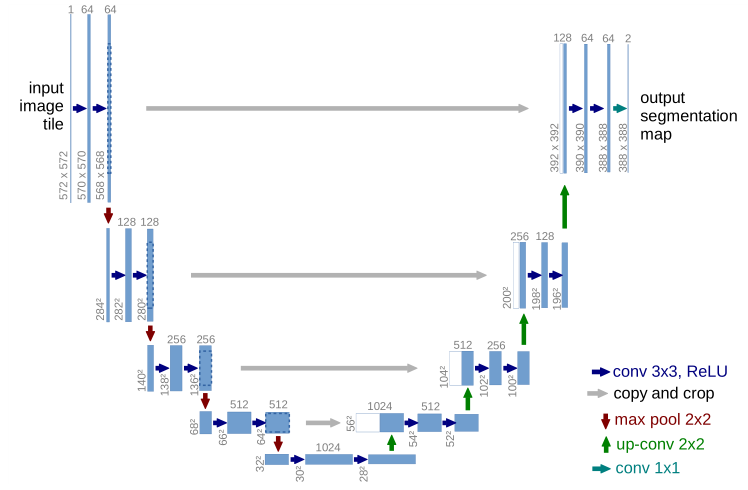
\includegraphics[width=.45\textwidth]{figures/U-Net_classic}
  \caption{U-Net architecture, taken from \cite{ronneberger2015}}
  \label{fig:two}
\end{figure}

% Norms
\begin{figure}[H]
  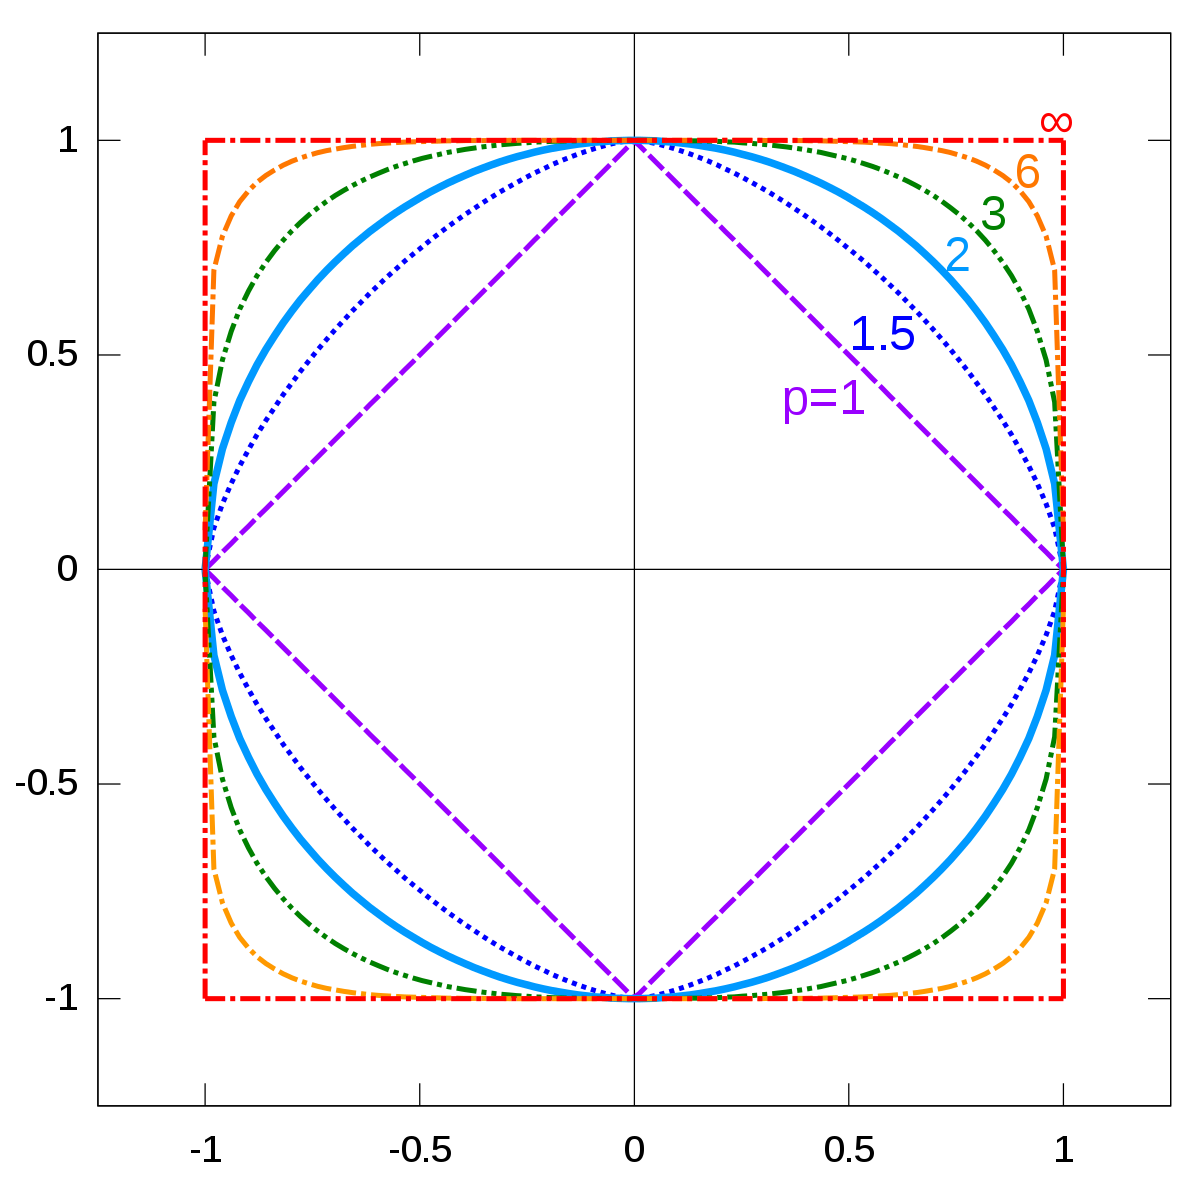
\includegraphics[width=.3\textwidth]{figures/norms}
  \caption{Vector norms visualized on unit circle, taken from \cite{norms_pic}}
  \label{fig:three}
\end{figure}

%%%%%%%%

% diff_bottleneck_conv
\begin{figure}[H]
  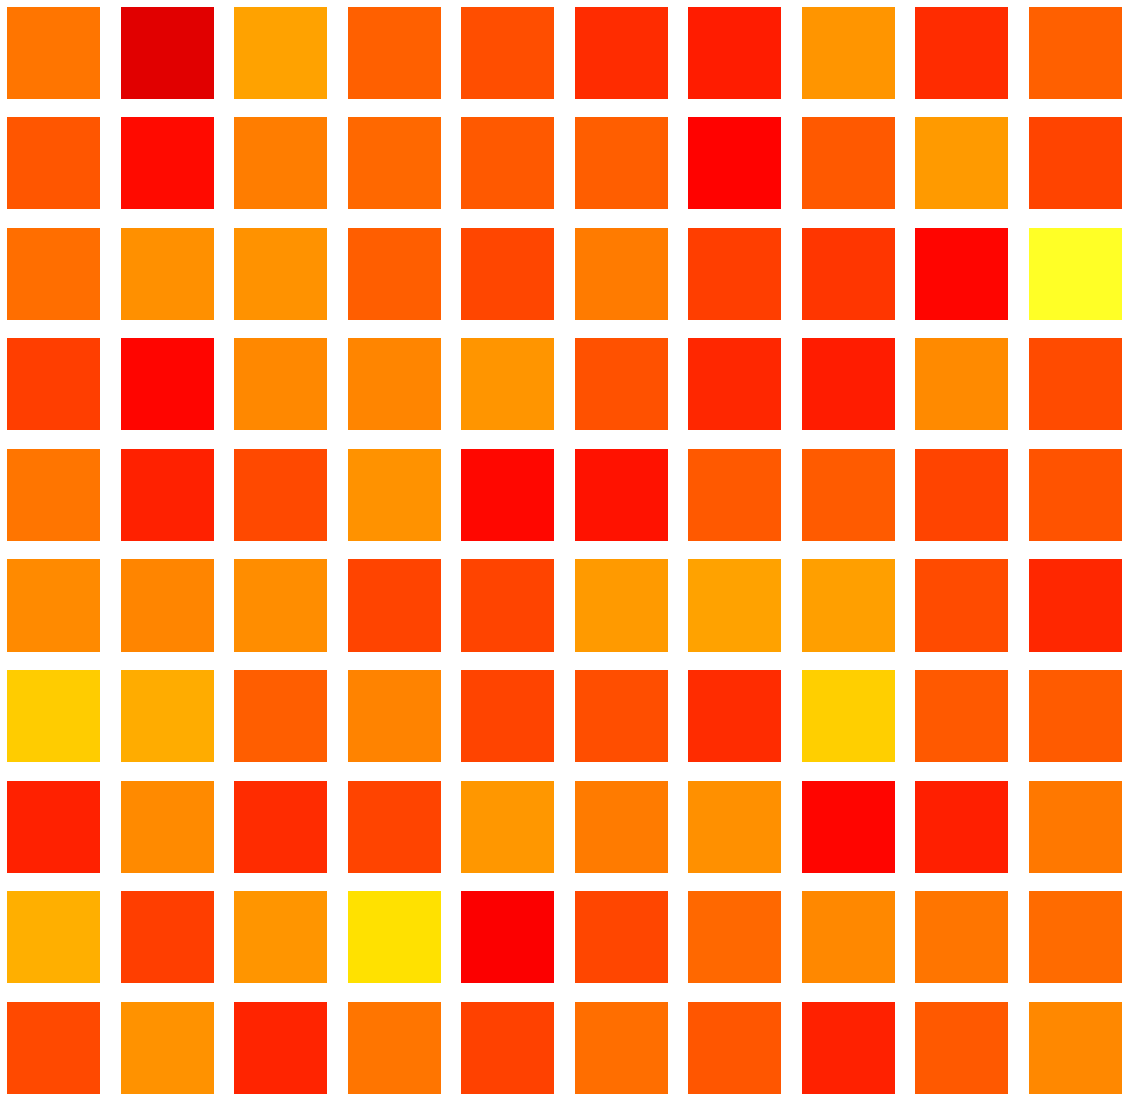
\includegraphics[width=.3\textwidth]{figures/weights_visualized/diff_bottleneck_conv.png}
  \caption{Convolution weight (bottleneck) difference between L1 and L2 normalization, first 100 weights.}
  \label{fig:four}
\end{figure}

\begin{comment}
% diff_layer_14_conv
\begin{figure}[H]
  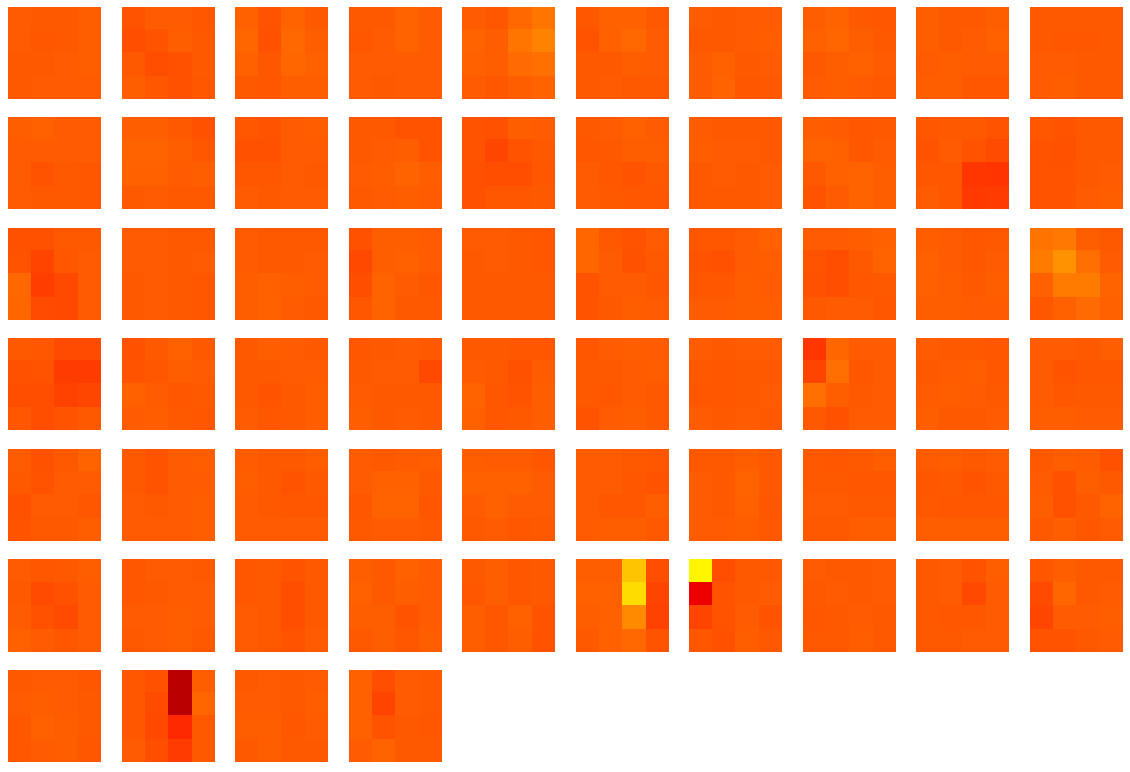
\includegraphics[width=.3\textwidth]{figures/weights_visualized/diff_layer_14_conv.png}
  \caption{}
  \label{fig:seven}
\end{figure}
\end{comment}




% Exact description of U-Net

\end{document}
